\chapter{Results}
\label{chap:results}


\section{hyperparameter gridsearch}

\begin{table}[h]
	\caption{
		Gridsearch MassSpecGym vs Gridsearch from this Thesis (lowest validation loss models in bold)
	}
    \resizebox{\textwidth}{!}{
	\begin{tabular}{p{6cm}W{c}{4cm}W{c}{4cm}}
		\toprule
                \textbf{Hyperparams} & \textbf{MassSpecGym} & \textbf{Thesis Gridsearch} \\
            \midrule
                Learning Rate & $\mathbf{3\cdot 10^{-4}}, 1\cdot 10^{-4}, 5\cdot 10^{-5}$ & $1\cdot 10^{-3}, 3\cdot 10^{-4}, \mathbf{1\cdot 10^{-4}}$\\
                Batch Size & $512, \mathbf{1024}$ & $\mathbf{512}, 1024, 2048$ \\
                $n$ predictions & $\mathbf{10}$ & $\mathbf{10}$ \\
                Transformer hidden dimensionality & $\mathbf{256}, 512$ & $\mathbf{128}, 256, 512$ \\
                Number of attention heads & $\mathbf{4}, 8$ & $2, 4, \mathbf{8}$ \\
                Number of encoding layers & $\mathbf{3}, 6$ & $\mathbf{2}, 3, 4$ \\
                Number of decoding layers & $\mathbf{4}$ & $2, 3, \mathbf{4}$ \\
		\midrule
	\end{tabular}}
	\label{tab:gridsearch}
\end{table}

\begin{figure}[h]
    \centering
    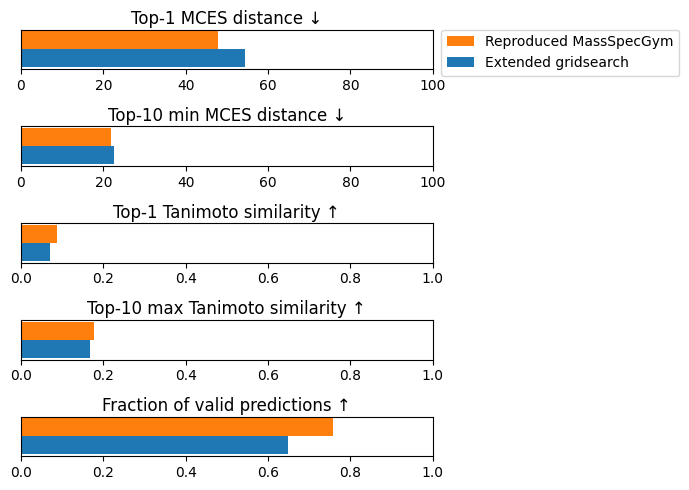
\includegraphics{figures/results/gridsearch_vs_paper.png}
    \caption{Evaluation SMILES model, retrained MassSpecGym vs best Gridsearch results based on validation loss}
    \label{fig:gridsearch_vs_paper}
\end{figure}

MCES distance, num valid mols voor modellen met naive sampler


\section{Samplers benchmark}


\section{\ac{BPE} as pretraining}


\section{Augmentation}

\subsection{SMILES augmentation}

\subsection{Spectral augmentation}


\section{Molecular representations benchmark}